\documentclass{article}
\usepackage{pgfornament}
\usepackage[english,greek]{babel}
\usepackage[utf8]{inputenc}
\usepackage[T1]{fontenc}
\pagestyle{empty}
\usepackage{tikz}
\usetikzlibrary{decorations.fractals}
\usepackage[papersize={,297mm}, strictheight=false,topmargin=0mm, botmargin, flap=50mm, textwidth=209mm, spine=13mm, cropmarks, cropframe, croptitle=croptitle]{zwpagelayout}
\usepackage{rotating}

\usepackage[final]{graphicx}
\usepackage{pdfpages}

\graphicspath{{images}}

\linespread{1}
\begin{document}
    \hbox to \textwidth{%
        \vbox to \textheight{\hsize \CropFlap \centering
        \textcolor{white}{Back flap}\vfill}\hss
        \vbox to \textheight{\hsize \UserWidth \vfill \leavevmode \textcolor{white}{ISBN+EAN}}\hss
        \vbox to \textheight{\hsize \CropSpine 
        \vspace{30mm}
        \begin{sideways}
            \hspace{-10cm} {\Large S.Fontana} \hspace{75mm} {\Large Relazione Finale} \hspace{75mm} {\Large A.A 2021/2022}}  
        \end{sideways}
    }\hss

    \vbox to \textheight{
        \hsize \UserWidth \vspace{1cm} 
        \setlength{\unitlength}{1cm}
        \begin{picture}(20,27)

            \put(65mm,222mm){
\includegraphics[height=30mm]{logo_unibs.png}}
            \put(70mm,187mm) {\fontsize{16}{10mm}\selectfont  \textbf{DIPARTIMENTO DI}}
            \put(40mm, 177mm) {\fontsize{16}{10mm}\selectfont \textbf{INGEGNERIA DELL'INFORMAZIONE}}
            
            \put(70mm,157mm) {\fontsize{17}{17}\selectfont CORSO DI LAUREA IN}
            \put(63mm, 147mm) {\fontsize{17}{17}\selectfont INGEGNERIA INFORMATICA}
            
            
            \put(75mm,127mm) {\fontsize{20}{20}\selectfont Relazione Finale}
            \put(33mm, 117mm) {\fontsize{20}{20}\selectfont \textbf{Sviluppo di un sistema di supporto alla}}
            \put(23mm, 107mm) {\fontsize{20}{20}\selectfont \textbf{programazione per dispositivi integrati della}}
            \put(75mm, 97mm) {\fontsize{20}{20}\selectfont \textbf{famiglia AVR}}
            
            \put(20mm, 70mm) {\fontsize{16}{16}\selectfont \textbf{Relatore}:}
            \put(20mm, 60mm) {\fontsize{16}{16}\selectfont Chiar.mo Prof. Alessandro Depari}
            
            \put(150mm, 50mm) {\fontsize{16}{16}\selectfont \textbf{Laureando}:}
            \put(142mm, 40mm) {\fontsize{16}{16}\selectfont Stefano Fontana}
            \put(133mm, 30mm) {\fontsize{16}{16}\selectfont Matricola n. 727199}
            
            \put(65mm, 10mm) {\fontsize{16}{16}\selectfont Anno Accademico 2021/2022}

            %\put(9.5,21) {{\Large CCC}}
            %\put(5.5,20.5) {{\Large DDD}}
            %\put(6,14){{\huge EEE \latintext{MicroMEGAS}}}
            %\put(7.5,7.5){{\Large FFF}}
            %\put(9,1.5){{\Large GGG}}

        \end{picture}}\hss
    \vbox to \textheight{\hsize \CropFlap \centering
    \textcolor{white}{Front flap}\vfill}}

    \newpage

    %\hbox to \textwidth{%
    %\vbox to \textheight{\hsize \CropFlap 
    %\vspace{20.5cm} 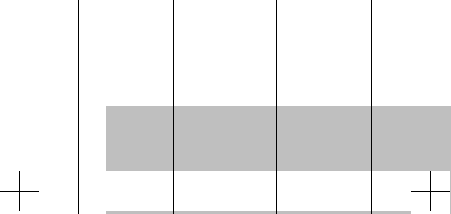
\begin{tikzpicture}\draw[color=gray!50,fill=gray!50] (0,0) rectangle     (5,-2);\end{tikzpicture}\vfill}\hss
    %\vbox to \textheight{\hsize \UserWidth \vspace{20.5cm}     \begin{tikzpicture}\draw[color=gray!50,fill=gray!50] (-2,0) rectangle     (30,-2);\end{tikzpicture}}\hss
    %\vbox to \textheight{\hsize \CropSpine \vfill
    %\begin{sideways}\hspace{-10cm}Αθανάσιος Ν. Σταματόπουλος  \hspace{5cm}{\Large Μελέτη     Ανιχνευτή \latintext{MicroMEGAS}}  \end{sideways}\vfill}\hss
    %\vbox to \textheight{\hsize \UserWidth \vspace{1cm} \line(1,0){40}{} \Large Σταματόπουλος     Ν. Αθανάσιος \line(1,0){320}\\ \setlength{\unitlength}{1cm}\begin{picture}(27,17)
    %\put(1,7){
\includegraphics[width=3.5cm]{logo_unibs.png}}
    %\put (5.5,9.5){\Large Εθνικό Μετσόβιο Πολυτεχνείο}
    %\put (5.5,9){\Large Σχολή Εφαρμοσμένων Μαθηματικών\&Φυσικών Επιστημών}
    %\put (5.5,8.5) {\Large Τομέας Φυσικής}
    %\put (5.5,8) {\Large Εργαστήριο Πειραματικής Φυσικής Υψηλών Ενεργειών}
    %\put (1,1) {\huge Μελέτη ανιχνευτή \latintext{MicroMEGAS}}\end{picture}
    %\begin{tikzpicture}
    %\draw[color=white,opacity=1] (0,2) -- (10,2);
    %\draw[color=gray!50,fill=gray!50] (0,0) rectangle (25,-2);
    %\node at (3,-6) {\large Οκτώβριος 2012};
    %\end{tikzpicture}
    %}\hss
    %\vbox to \textheight{\hsize \CropFlap \vspace{20.5cm}     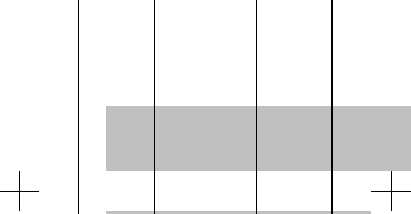
\begin{tikzpicture}\draw[color=gray!50,fill=gray!50] (0,0) rectangle     (4.5,-2);\end{tikzpicture}\vfill}}
%
\end{document}